\documentclass{mcmthesis}
\bibliographystyle{unsrt}
\mcmsetup{CTeX = false,   % 使用 CTeX 套装时,设置为 true
        tcn = 1925307, problem = E,
        sheet = true, titleinsheet = true, keywordsinsheet = true,
        titlepage = false, abstract = true}
\usepackage{palatino}
\usepackage{lipsum}
\usepackage[UTF8, nocap]{ctex}
\usepackage{array}
\usepackage{float}
\usepackage{booktabs}
\usepackage{multirow}
\usepackage{subfigure}
\usepackage{longtable}
\usepackage{setspace}
%\usepackage{ctex}
%\usepackage{CJK}
\title{Putting Environmental Costs on the Balance Sheet!}
\author{}
\date{\today}

\begin{document}

	\begin{abstract}
		
		Ecological economics has challenged traditional methods of traditional natural resources. In recent years, the monetary value of biodiversity and ecosystem services has often been seen as a crucial process affecting economic decision-making. We establish a valuation model to measure the environmental cost of the land-use project. Then it is applied to Beijing and a waste-to-power plant to show their environmental cost. At last, we discuss the implication on planners and managers, and how might the model need to changes over time.
		
		Our environmental cost valuation model provides a quantitative analysis based on monetary measurement. It considers multiple aspects, including ecosystem services and environmental degradation. We use nine indicators to measure every three aspects of ecosystem services. We use various methodologies to quantify each indicator. Moreover, we have further regulated it with biodiversity by interacting with ecosystem services. The effects of Environmental degradation is divided into two parts: Biodiversity loss and Pollution. Biodiversity directly impacts the degradation as a service. And we use three indicators to represent the influences of water, air and solid waste pollution.
		
		We choose Bejing and a waste-to-energy plant in our cases study. We found that the main cost of community-based projects is mainly from pollution, while the national project' is the consumption of ecosystem services. What's more, also it can be seen that Beijing has made efforts to protect the environment.
		
		Furthermore, we discuss the implications on project planners and managers. Planners can use our model to find the most appropriate site. Based on the production possibility boundary theorem, managers can use our model to find the most valuable projects combinations.
		
		As time goes by, more and more governments start to take environmental costs into account. In this paper, we mainly discuss how Pigovian tax and Politics of Tradeable Pollution Rights will affect our model, and analyze how might our model need to change over time.
		
		Finally, we conduct a sensitivity analysis to gain some deep understanding of our model and conclude the paper via discussing the strengths and weaknesses of our model.
		
		
		\begin{keywords}
			Ecosystem services; Evironmental cost, Biodiversity, Pollution
		\end{keywords}
	\end{abstract}

	\maketitle
	\setcounter{tocdepth}{2}
	\tableofcontents
	
	
	\section{Introduction}
	
		\subsection{Background}
		
			In a certain historical period, economic growth has played a huge role in improving people's living standards and national welfare, but economic growth is not costless, and environmental destruction is one of its main costs. These environmental damages lead to a reduction in the ecosystem services supply, which also leads to an environmental degradation.
			
			For a country, when the marginal cost of economic growth exceeds its marginal benefit, this economic growth is diseconomy \cite{daly1997beyond}. For a land use project, it is also diseconomical when the cost including the environmental costs is greater than the revenue. Therefore, it makes great sense to incorporate environmental costs into the economic accounting system.
			
			The economic accounting model for environmental costs of land use project is still in dispute \cite{plumecocq2014second}. We, the ICM team, trying to find a solution, faces the problems below:
			\begin{itemize}
				%\addtolength{\itemsep}{-1.5ex}
				\item Create an ecological services valuation model taking ecosystem services into account to understand the real economic costs of land use projects.
				
				\item Perform a cost-benefit analysis of varying size project, from small community-based projects to large national projects. 
				
				\item Evaluate the effectiveness of our model based on your analyses and model design. 
				
				\item Consider implications of our modeling on
				land use project planners and managers.
				
				\item Explore the possible changes of the model over time.
			\end{itemize}
		
		\subsection{Literature Review}
			After realizing the contribution of ecosystem bring to human welfare researchers have estimated the current economic value of ecosystem services non-systematically \cite{costanza1997value}. The proposal of System of Integrated Environmental and Economic Accounting (SEEA)\footnote{The System of Environmental-Economic Accounting 2012 — Central Framework (SEEA Central Framework) is a statistical framework consisting of a comprehensive set of tables and accounts, which guides the compilation of consistent and comparable statistics and indicators for policymaking, analysis and research.} and The Economics of Ecosystems and Biodiversity (TEEB)\footnote{The Economics of Ecosystems and Biodiversity (TEEB) is a global initiative focused on making nature’s values visible and its principal objective is to integrate the values of biodiversity and ecosystem services into economic decisions.} is a response to the shortcomings of traditional accounting methods. After that, some people applied those frameworks to various government levels \cite{dalmazzone2013multi} and several scarce resources such as water \cite{pedro2016use}.
			
			We expect to quantify the impact of ecological degradation on computing environmental costs and integrate environmental cost into land-use projects base on the previous wisdom and necessary methodologies.
			
		\subsection{Analysis and Approach Overview}
			
			Since the impact of human activities on the environment is so dramatic that we have to pay attention to the consumption of the environment. It is significant to propose an efficient model to understand the true economic costs of land-use projects when ecosystem services and environmental degradation are considered. We aim to design a measuring system to quantify the environmental costs. Two specific projects are selected to perform benefit-cost analyze with the environmental costs calculated by our model. Then we have to discuss the implications of our model on planners and managers. Eventually, we need to make sure what change should be executed to our model over time.
			
			Through the above analysis, the flow chart of this paper is shown in Figure \ref{fig:flowchart} as follows:
			
			\begin{figure}[h]
				\small
				\centering
				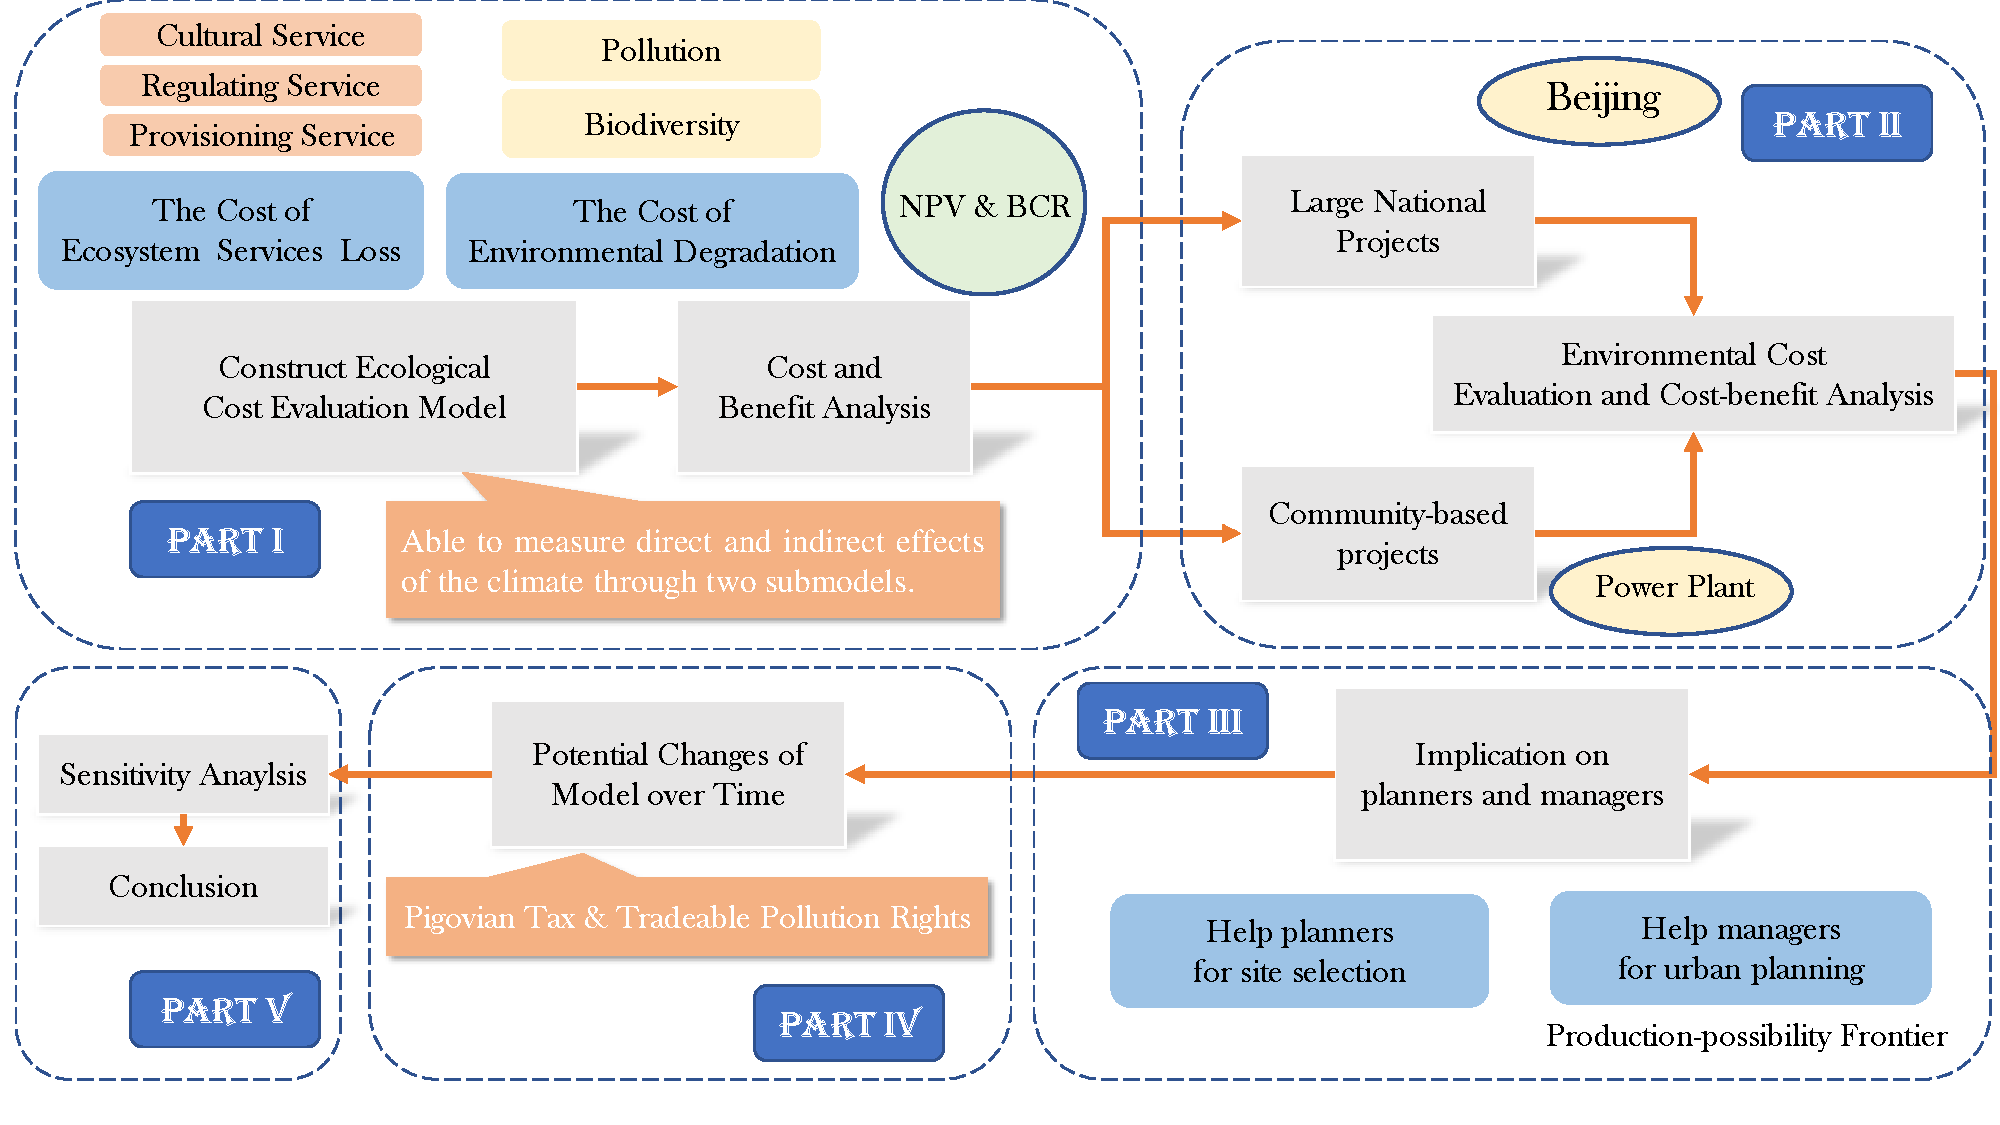
\includegraphics[width=14cm]{flowchart.pdf}
				\caption{The flow chart in this paper}
				\label{fig:flowchart}
			\end{figure}

		
	\section{Preliminaries}
		\subsection{Main Assumptions}
		
			\begin{itemize}
				\item \textbf{There are limits to the demand for earth resources \cite{rockstrom2009safe}}.  \\ 
				Due to the planet boundaries \footnote{Planetary boundaries define the safe operating space for humanity with respect to the Earth system and if these thresholds are crossed, then important subsystems could shift into a new state, often with deleterious or potentially even disastrous consequences for humans.}, the environment is a scarce resource essentially, and it has economic value as well.
				
				\item \textbf{The value of the environment is not fully reflected in the market.}\\
				There is a negative externality in the use of ecosystem resources, that is, environmental costs are not truly included in economic costs.
				
				\item \textbf{Ignore inflation and deflation of money.} 
				\\The value of money remains unchanged.
				
				\item \textbf{Project land loses all of its value of ecosystem services.} \\
				If the land used for the project is forest, mountain, wetland and other ecological sites, then all of its ecosystem services will be lost. Land in urban have no ecosystem services.
				
				
			\end{itemize}
		
		\subsection{Notations}
		
			In order to be clear and consistent through the paper, we now settle down some terms	and mathematical notations:
			
			\begin{table}[h]
				\caption{Symbol Table}
				\centering
				\renewcommand\arraystretch{1.32}
				\begin{tabular}{c l}
					\hline
					Symbol & Definition\\
					\noalign{\global\arrayrulewidth1pt}\hline\noalign{\global\arrayrulewidth0.9pt}

					Provisioning& 	Provisioning Services Cost\\
					$P_{cons}$&	the economic cost of the annual water-conservation capacity of the area\\
					$P_{wast}$&	the value of reduced waste lands \\
					$P_{land}$&	the economic benefits of maintaining soil fertility \\
					$P_{send}$&	the economic benefits of reducing sediments deposit\\
					Regulating&	Regulating Services Cost\\
					$R_{carb}$&	the annual carbon fixation value of the area\\
					$R_{oxyg}$&	the annual oxygen release value of the area\\
					$R_{anion}$&	the anion value provided by the area\\
					$R_{sulf}$&	the annual absorption value of the area\\
					Culture&	Cultural Services Cost\\
					$V_{WTP}$&	value of the willingness to pay\\
					$V_{ATP}$&	value of the ability to pay\\
					Us&	the value of protecting species of area\\
					Pollution&	the economic cost of pollution\\
					$V_{iw}$&	the cost of water pollution \\
					$V_{ig}$&	the cost of industry air pollution\\
					$V_{ug}$&	the cost of urban life air pollution\\
					$V_{sw}$&	the cost of solid waste pollution\\
					NPV&	the net price value in cost-benefit analysis\\


					\hline
					
				\end{tabular}
			\end{table}
			
	
	\section{Environmental Cost Valuation Model}
	
		The unconventional characteristic of this report's model comes from its derivation. The monetary measurement methods are used to measure the environmental costs, so there is no need for the weighting process. In the assessment of the environmental cost of a land use project, We classify the environmental cost into two main parts: Cost of ecosystem services loss and Cost of pollution, and we will demonstrate the quantitation analysis of them respectively.
		
		
		\begin{figure}[h]
			\small
			\centering
			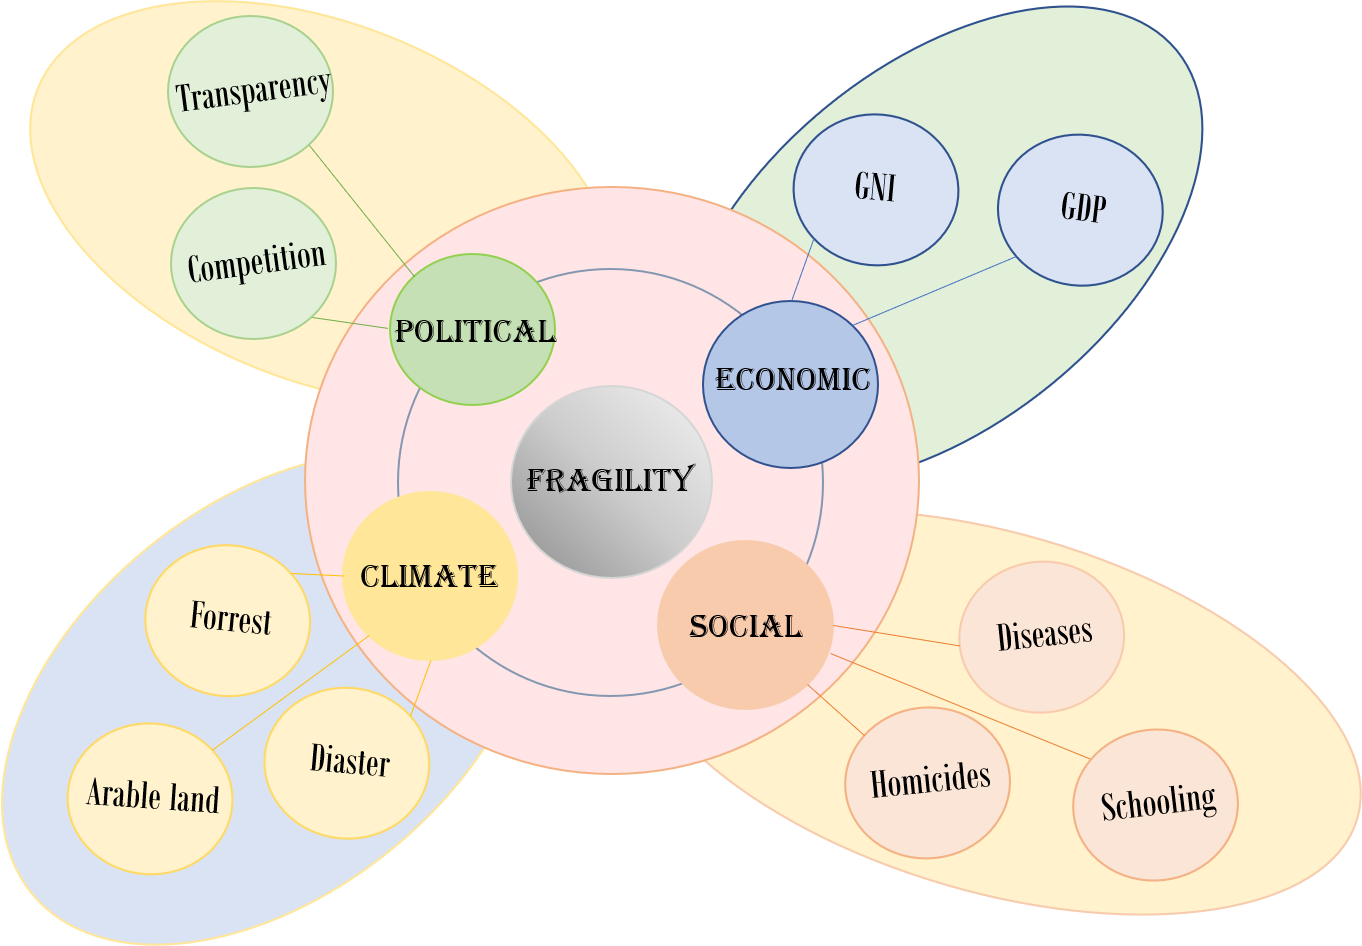
\includegraphics[width=15cm]{over-all.png}
			\caption{Framework of Environmental Cost Valuation Model}
			\label{fig:over-all}
		\end{figure}
	
		\subsection{The Cost of Ecosystem Services Loss}
		
			Under the guide of Ecosystem Services \cite{assessment2005millennium}, we classify the factors into three main fields: provisioning services, regulating services and cultural services. Factors in separate fields contribute to environment cost in diverse ways. We introduce the quantification of impact from various actors field by field. The quantification of every factor's impact will be presented below.
	
			\subsubsection{Provisioning services}
			
				We use four provisioning services indicators in this field. These four indicators measure the decline of the potential material benefits people can obtain from ecosystems.
				
				Product Amount Method (PAM) and Value Amount Method (VAM) are selected to cope with the quantification process. These two methods comprehensively assess the services provided by the ecosystem from the perspective of product amount and the value amount respectively \cite{zhiming2017valuation}.
				
				\begin{itemize}
					
					\item \textbf{Conservation of water} \\
					Conservation of water measures the value of holding-water and the value of reducing the peak flow, lagging of flood time and supplying water in dry season.
					
					\begin{equation}
						P_{cons} = W \times P = ( R - E ) \times A \times P
					\end{equation}
					
					where $W$ is the water-conservation capacity ($m^3$); $R$ stands for the annual amount of precipitation ($m^3$); $E$ is the average annual evapotranspiration ($mm$) of the area; $A$ means the wood land area ($hm^3$); $P$ is the water storage cost per unit ($\$/m^3$)
					
					\item \textbf{Reduced waste lands} \\
					Reduced waste lands plays an important role in soil conservation. This indicator measures the cost of ecosystem’s loss for reducing waste lands.
					
					\begin{equation}
					\begin{array} { l } 
					{ P _ { wast } = \frac { ( V \times B ) } { ( 10000 \times L \times D ) } } \\ 
					{ V = S \times ( P - Q ) } 
					\end{array}
					\end{equation}
					
					where $V$ is the reduced soil erosion amount ($t/year$); $D$ stands for the average density of soil ($t/m^3$); $L$ is the forest soil thickness ($t/m^3$); $B$ is the average benefits of forestry ($\$/hm^2$); $S$ means forest area ($hm^2$); $P$ is the modulus of potential soil erosion ($t/(hm^2 ·year)$); $Q$ is the modulus of realistic soil erosion ($t/(hm^2 ·year)$)
					
					\item \textbf{Land fertility}\\
					Nutrients such as N, P and K in soil runoff because of land use. The ability to keep land fertility also plays a significant role in soil conservation. This indicator measures the cost of losing land fertility conservation.
					
					\begin{equation}
					P _ { land } = \sum V \times C _ { i } \times \frac { P } { 10 } \times 1000 ( i = N , P , K )
					\end{equation}
					
					where $C_i$ is the net contents of $N$, $P$, and $K$ in soil; $P$ is the price of $N$, $P$, $K$ (\$).
						
						
					
					\item \textbf{Reduced sediments in rivers}. \\
					According to the law of sediment movement, a lot of erosive soils are deposited in reservoirs, rivers, and lakes. It measures the cost of reducing sediments in rivers.
					
					\begin{equation}
					P _ { send } = \frac { P \times V \times U } { 10000 }
					\end{equation}
					
					\noindent
					where $U$ stands for the costs of reservoir project ($\$$). $P$ is the percent of the erosive soils that are deposited in reservoirs, rivers, and lakes.
					
				\end{itemize}
			
				The mathematical expression for provisioning services indicators in the environmental cost valuation model has a form of
				
				\begin{equation}
					Provisioning = P_{cons} + P_{wast} + P_{land} + P_{send}
				\end{equation}
			
			
				
			\subsubsection{Regulating services}
			
				We use two Regulating services indicators in this field. These two indicators measure the loss of the value of air and soil, providing flood and disease control, or pollinating crops.
				
				
				\begin{itemize}
					
					\item \textbf{Carbon fixation and oxygen release} \\
					Carbon fixation and oxygen release refers to the fixation of carbon and release of oxygen. These two indicators represent the cost of losing carbon fixation and oxygen release ability.
					
					\begin{equation}
						\begin{aligned} 
						R _ { carb } & = A _ { i } \times C _ { c } \left( 63 \times R _ { c } \times B _ { n } + F _ { c } \right) \\ 
						R _ { oxyg } & = 1.19 \times A _ { i } \times C _ { c } \times B _ { n } \end{aligned}
					\end{equation}
					
					where $C_c$ is the price of fixed carbon, and $C_o$ is the price of oxygen, yuan/year; $R_c$ is the carbon content in CO2 (taking 27.27\%); $B_n$ is the annual net productivity of the area, and $F_c$ is the annual carbon content per unit area of the area, ($t/(hm^2 ·year)$).
					
					\item \textbf{Purification of the air} \\
					Purification of the air refers to the ability of absorbing sulfur dioxide, fluorine, nitrogen oxides and the ability of reducing noise and detaining dust of the area. Now we use from 0 to 6 to represent anion, sulfur dioxide, fluoride, nitrogen oxides, dust retention and noise.
					
					
					
					\begin{equation}
					\begin{array} { l } 
					{R _ { anion } = [ 5.256 \times 10 ^ { 15 } \times A _ { i } H K _ { i } \left( Q _ { i } \right) ] / L  }\\ 
					{ R _ { sulf } = \sum _ { i = 1 } ^ { 5 } A _ { i } K _ { i } Q _ { i }} 
					\end{array}
					\end{equation}
					
					where $H$ is the height of the area ($m$); $Qi$ represents the amount absorbed by the area per unit area [$kg/(hm^2·a)$]. $Ki$ represents the cost ($\$/kg$), but $K_0$ is the cost generated by an anion ($\$/one$); $L$ is the life time of an anion ($min$); $A_i$ is the size, but $A_5$ is the mile of sound-proofing walls converted from forest area ($km$);
					
	
				\end{itemize}
				
				The mathematical expression for regulating services indicators in the environmental cost valuation model has a form of
				
				\begin{equation}
				Regulating = R_{carb} + R _ { oxyg } + R_{anion} + R_{sulf}
				\end{equation}
				
			\subsubsection{Cultural services}
			
				Cultural services measure the loss of the non-material benefits people obtain from ecosystems. It will be measured in terms of willingness to pay(WTP) and ability to pay(ATP). Conditional valuation method (CVM) is widely used in valuing environmental goods and services in terms of willingness to pay \cite{mitchell2013using}.
				
				Average willingness to pay is calculated as follow:
				
				\begin{equation}
					\begin{array}{ l } 
					{E ( W T P ) = \sum _ { i = 1 } ^ { n } P _ { i } A _ { i }}\\
					{V _ { W T P } = E ( W T P ) \times N}
					\end{array}
				\end{equation}
				
				Where $A_i$ is the bidding value that the respondent will pay. $P_i$ is the probability that the respondent chooses this tender value. $n$ is the number of bids; $N$ is population.
				According to econometric theory, we adopt extended linear expenditure system (ELES) model to measure people’s ability to pay.
				
				\begin{equation}
				\begin{array} { l } { p _ { i } q _ { i } = p _ { i } r _ { i } + \beta \left( I - \sum _ { j } ^ { n } p _ { j } r _ { j } \right) } \\ { V _ { A T P } = \sum _ { i = 1 } ^ { n } p _ { i } q _ { i } } \end{array}
				\end{equation}
				
				
				
				Where, $i$ is the category of consumer expenditure; $n$ is the total number of categories; $q_i$, $r_i$ and $β_i$ are the actual demand, basic demand and marginal propensity to consume of consumers for the ith commodity or service.  $p_i$ is the price of the ith commodity or service; $I$ is consumer income.
				
				No one can pay more for a product than they can afford, and no one are willing to pay more for a product than their willingness. So the value of ecosystem cultural services is determined by the minimum value of $V_{WTP}$ and $V_{ATP}$. It’s show as follow:
				
				\begin{equation}
					Culture = \min \left( V _ { W T P } , V _ { A T P } \right)
				\end{equation}
				
				
		\subsection{Environmental Degradation}
		
			\subsubsection{Environmental degradation caused by biodiversity loss}
			
				There is a positive relationship between biodiversity and most ecosystem services. Biodiversity has multiple roles in the delivery of ecosystem services, as a regulator of ecosystem processes, as the service and good \cite{mace2012biodiversity}.
	

				
				\subsubsection{Biodiversity Regulator}
				
					The extent of human impact on an ecosystem is a key factor in assessing the provision of different categories of ecosystem services \cite{cimon2013fostering}. In this paper, we mainly talk about the land use projects' impact on ecosystem, and they cause change on ecosystem services by impacting the biodiversity directly. \cite{de2010challenges} Biodiversity plays an important role in regulating ecosystem services, which means that it can buffer environmental changes and maintain ecosystem services in the face of disturbance. The prevailing view is that when biodiversity is lost, ecosystems become less resilient, so the sum provision of different categories of ecosystem services is impacted by the varying degrees of biodiversity.
					
					
					Biodiversity is divided into six categories according to human intervention: Natural, Light use, Extensive, Intensive, Degraded and Urban. Generally speaking, every categories’ effect is similar, and each of them has the same impact on ecosystem services, based on the data from literature \cite{de2010challenges}, let $R$ denote the biodiversity regulator.
					
				
				\subsubsection{Biodiversity service and good}
				
					We make a reasonable assumption that individuals in aggregate would be willing to incur these costs if the natural services were no longer available.
					
					When biodiversity plays as goods or plays as a kind of ecosystem services, it’s a direct component of ecosystem service cost when running a land use project. To measure this direct cost, replacement/restoration cost technique is our best choice. The restoration cost (RC) approach assesses the value of an ecosystem service by how much it costs to replace/restore it after it has been damaged \cite{garrod1999economic}.
					
					\begin{equation}
						U _ { s } = S _ { s } \times A _ { i }
					\end{equation}
					
					\noindent
					where $S_s$ is the annual opportunity cost of lost forest species per unit area ($(yuan/(hm^2·a)$).
					
			\subsubsection{Environmental degradation caused by Pollution}
				
				If all pollutants are treated, environmental degradation will not occur so badly. The economic value of environmental degradation already occurring should be the cost of treating all pollutants. To measure the economic more accurately, we divide pollution into \textbf{water pollution}, \textbf{air pollution} and \textbf{solid waste pollution} to calculate each economic value of them.
				
				\begin{itemize}
					
					\item \textbf{Cost of water pollution}
					
					The cost of pollutant treatment for industry and urban life are both taken into account. The pollutants in industrial wastewater include COD, ammonia nitrogen, hydride, petroleum and heavy metals. Domestic wastewater includes tertiary industry wastewater and residential wastewater, and the treatment cost of each part is composed of COD treatment cost and ammonia nitrogen treatment cost.
					
					The formula for calculating the cost of treating water pollution is as follows
					
					\begin{equation}
						V _ { i w } = \sum _ { i = 1 } ^ { 7 } \left( A _ { i } \times C _ { i } \times r _ { i } \right)
					\end{equation}
					
					where $A_i$, $C_i$ and $r_i$ represent each pollutants’ emissions, unit governance cost and removal.
					
					\item \textbf{Cost of air pollution}
					
					We consider air pollution comes from industry and urban life. The pollutants in industrial gas include $SO_2$, dust, $NO_x$. The formula for calculating the cost of treating industrial is as follows
					
					\begin{equation}
						V _ { i g } = \sum _ { i = 1 } ^ { 3 } \left( A _ { i } \times C _ { i } \times r _ { i } \right)
					\end{equation}
					
					where $A_i$, $C_i$ and $r_i$ represent each pollutants’ emissions, unit governance cost and removal.
					
					Urban life air pollution comes from the fuel gas including Natural gas, gas and liquefied petroleum gas, the formula for calculating the cost of treating industrial is as follows
					
					\begin{equation}
						V _ { u g } = \sum _ { i = 1 } ^ { 3 } \left( N \times p _ { i } \times C _ { i } \right) + C _ { h }
					\end{equation}
					
					where $N$ is the city’s population,$pi$ is gas usage ratio,$Ci$ is Per capita gas use cost,$Ch$ is Heating costs, $I$ represents three kinds of gas.
					
					
					\item \textbf{Cost of solid waste pollution}
					
					Solid waste includes industrial solid waste and municipal solid waste. Industrial solid waste consists of two parts, a waste of storage and discharge. Their treatment cost can be calculated in the same way; the formula is shown as follow:
					
					\begin{equation}
						V _ { sw } = A \times C
					\end{equation}
				
					where $A$ represents discharge or storage capacity,$C$ stands unit processing costs.

				\end{itemize}
			
				So the total cost of pollution caused by land-use project is 
				
				\begin{equation}
				Pollution = V _ { i w } + V _ { i g } + V _ { u g } + V _ { sw }
				\end{equation}
				
		
		\subsection{Calculation}
			
			The outcome of ecological services valuation model shows the environmental costs of a land project. The model has the equation form as:
			
			\begin{equation}
			\operatorname { Cost } = \frac { \text { Regulating } + \text { Provisioning } + \text { Culture } } { R } + U _ { s } + \text { Pollution }
			\end{equation}
			
			Equation shows the environmental cost that a land use project doesn’t consider. It contains ecosystem services part and environment degradation part. Ecosystem services include Supporting services, Provisioning services, Regulating services and Cultural services. Biodiversity has a role as a regulator, which is a big part of supporting services, so we use biodiversity instead of supporting services. Environment degradation consists of Pollution and some part of Biodiversity. Bigger value of the indicators, bigger the environmental costs.
			
			
			
	\section{Cost-benefit Analysis Model}
	
		Cost analysis method is mainly used to calculate the net present value(NPV) and benefit-cost ratio, then select the best project by comparing all of the options. 
		
		Objectively, land use projects can produce two different kinds of effects. One kind is internal effect, point to the expenditure that belongs to development land itself to go up economically and accrual, expression is internal cost and internal benefit. The other is the external effect, which refers to the positive and negative effects of land development and utilization on surrounding resources and environment. Traditionally, most land use projects only consider internal costs and benefits, but ignore the external costs. Then it causes a lot of ecological problems, and destroyed the overall development of agriculture and the virtuous cycle of ecological and economic system, results in great external costs. That’s why we should take external costs into cost-benefit analysis (CBA).
		
		\subsection{Costs and Benefits Analysis}
		
			\subsubsection{Costs}
			
				The costs of land use projects can be classified as internal costs and external costs.
				
				\begin{itemize}
					
					\item \textbf{The external costs.}
					
					The external costs are not directly shown as expenditures on land use but as a monetary estimate of the loss of its other environment arising from the development of the land. Based on our ecological services valuation model, we can calculate the specific external costs of this project.
					
					\item \textbf{The internal costs.}
					
					The internal cost is the direct expense incurred by the land use project. It includes the investment in land use, operating expenses for land use and so on. These costs can be obtained from statistics.
					
				\end{itemize}
					

			\subsubsection{Benefits}
			
				The benefits of land use projects can be classified as internal benefits and external benefits. Usually land use projects do not produce external benefits, so we don’t take external benefits into consideration. internal benefits are the benefits resulting from land use that can be estimated directly from market prices. They’re the direct results of the land use projects.
		
		
		\subsection{Calculation}
		
			We use two indicators for cost-benefit analysis: Net Present Value(NPV) and Benefit-cost Ratio(BCR). The two indicators have both goodness and shortcoming. When analysing projects of the same size, they have the same function. But when considering projects of different scales at the same time, the NPV method is more inclined to choose large-scale projects, while the rate is more willing to select small-scale projects.
			
			\begin{itemize}
				
				\item \textbf{NPV}
				
					\begin{equation}	
						N P V = \frac { B } { 1 + r } - C _ { i } - C _ { e }
					\end{equation}
					
					where $B$ is benefits, $C_i$ is internal costs, $C_e$ is external costs, $r$ is the discount rate.
				
				\item \textbf{BCR}				
					\begin{equation}
						K = \frac { \frac { B } { 1 + r } } { C _ { i } + C _ { e } }
					\end{equation}
					
					where $B$ is benefits, $C_i$ is internal costs, $C_e$ is external costs, $r$ is the discount rate.
				
			\end{itemize}
		
	%\clearpage

	\section{Analysis for Two Projects}
	
		\subsection{Community-based Project: Xiaogan Waste-to-Energy Plant}
		
		Data collection is the basis for project analysis. Our data source has two parts: statistical data and remote sensing data. We searched the statistical data on the Municipal Bureau of Statistics and selected two projects with the complete data for analysis. Remote sensing data comes from the National Earth System Science Data Sharing Infrastructure.
		
		Xiaogan is a central city of Hubei Province, China. We choose the waste-to-energy plant in Xiaogan as our community-based project. The plant generates electricity by burning garbage, and it generates electricity while solving the problem of municipal waste. This way of treating garbage is highly respected by the government.
		
		
		Total investment of Xiaogan Waste-to-Energy Plant is about 126.3 million dollars, and it covers an area of 87,096 square meters built on cultivated land. The annual power grid of the plant is 1.815×108 kWh.
		
		\begin{figure}[h]
			\small
			\centering
			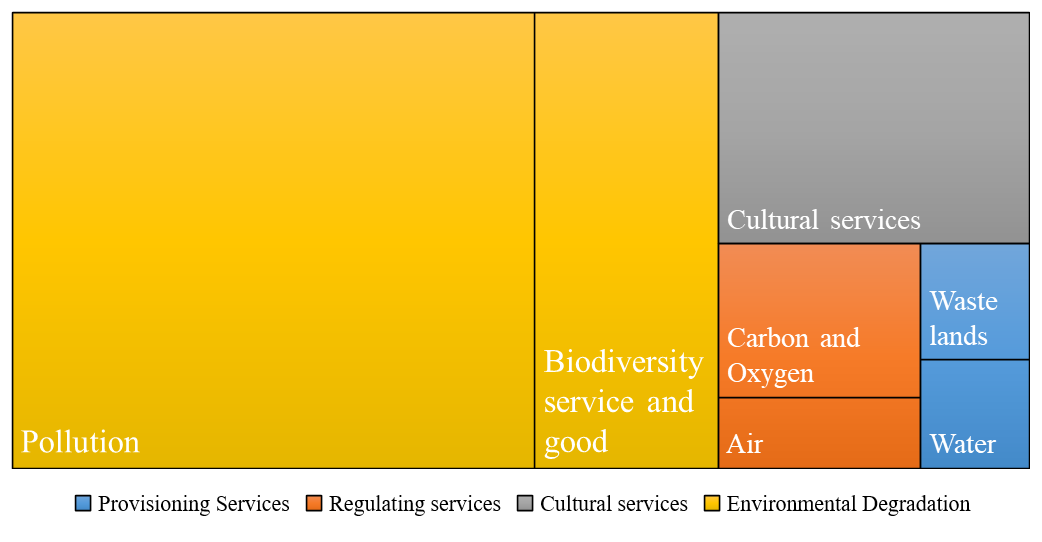
\includegraphics[width=14cm]{community.png}
			\caption{Community-based project: Xiaogan Waste-to-Energy Plant}
			\label{fig:community}
		\end{figure}
	
		According to the figure \ref{fig:community}, we have following conclusions: for this community-level land use project, most of the environmental costs come from environmental degradation, with pollution accounting for a large part. And the reduction in ecosystem services is not significant.
		
		\begin{table}[h]
			\centering
			\label{Ecological-Cost}
			\caption{Cost-benefit Analysis}
			\setlength{\tabcolsep}{3.7mm}
			\begin{tabular}{ccc}
				\toprule[1.5pt]  %添加表格头部粗线
				Methods & Without Ecological Cost & With Ecological Cost  \\
				\midrule  %添加表格中横线
				NPV & 1817383 dollars & 668300 dollars  \\
				BCR & 1.22 & 1.07  \\
				\bottomrule[1.5pt] %添加表格底部粗线
			\end{tabular}
		\end{table}
		
		From the results of table 1, we can see that the ecological cost of the plant is 114.9 thousands of dollars. When the ecological cost is not considered, the Benefit-cost Ratio of the project is 1.22, but after the ecological cost is considered, the Benefit-cost Ratio of the project becomes 1.07. When the ecological costs are not taken into account, the project is highly commendable, but when we calculate the ecological costs, the project is not as good as expected.
		
		
		\subsection{Large National Project:  Beijing}
		
		When we are considering large national projects, we think that the development of each city is the use of land resources. The rapid development of a city means the use of environmental resources and the subsequent environmental degradation. We want to study the ecological cost of a city by analyzing the development of it.
		
		We chose Beijing, the capital of China, as the city we studied. The total area of Beijing is 16,410.54 square kilometers, As the capital of China, Beijing develops rapidly, but at the same time, there are many environmental problems. In recent years, the government has begun to pay attention to environmental problems and has taken many measures.
		
		\begin{figure}[htbp]
			\centering
			\subfigure[2010]{
				\begin{minipage}[t]{0.5\linewidth}
					\centering
					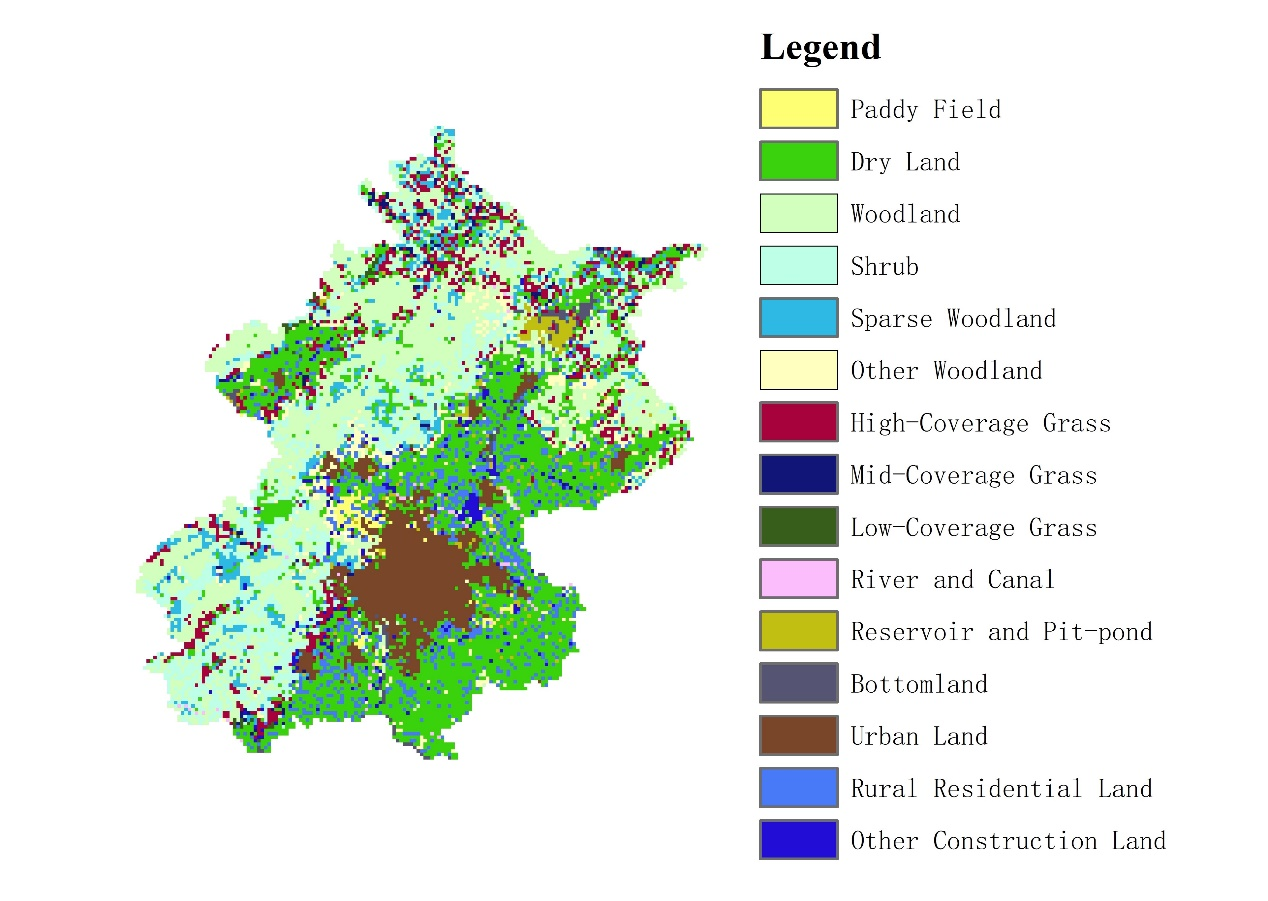
\includegraphics[width=3in]{map.png}
					%\caption{fig1}
				\end{minipage}%
			}%
			\subfigure[2015]{
				\begin{minipage}[t]{0.5\linewidth}
					\centering
					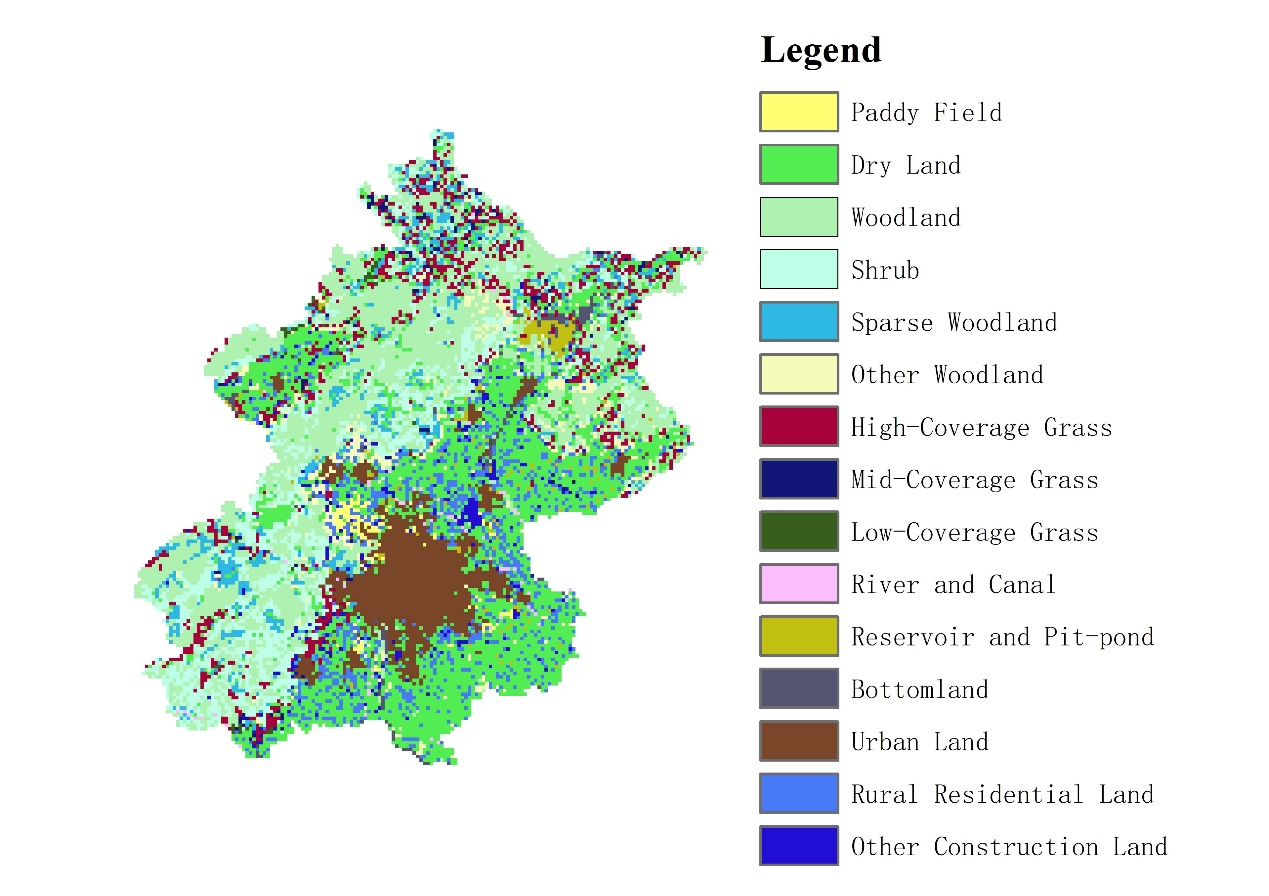
\includegraphics[width=3in]{map2.png}
					%\caption{fig2}
				\end{minipage}%
			}%
			\centering
			\caption{The Land Use of Beijing in 2010 and 2015}
		\end{figure}
		
		
		
		These two figures below show the land use of Beijing in 2010 and 2015 respectively, from which we can see the slow degradation of the environment caused by the development process.
		
		From the statistics, we can see that due to the increasing emphasis on environmental issues by the government, although the area of cultivated land, garden land, woodland and grassland is still decreasing every year, the reduction is decreasing year by year.
		
		\begin{figure}[h]
			\small
			\centering
			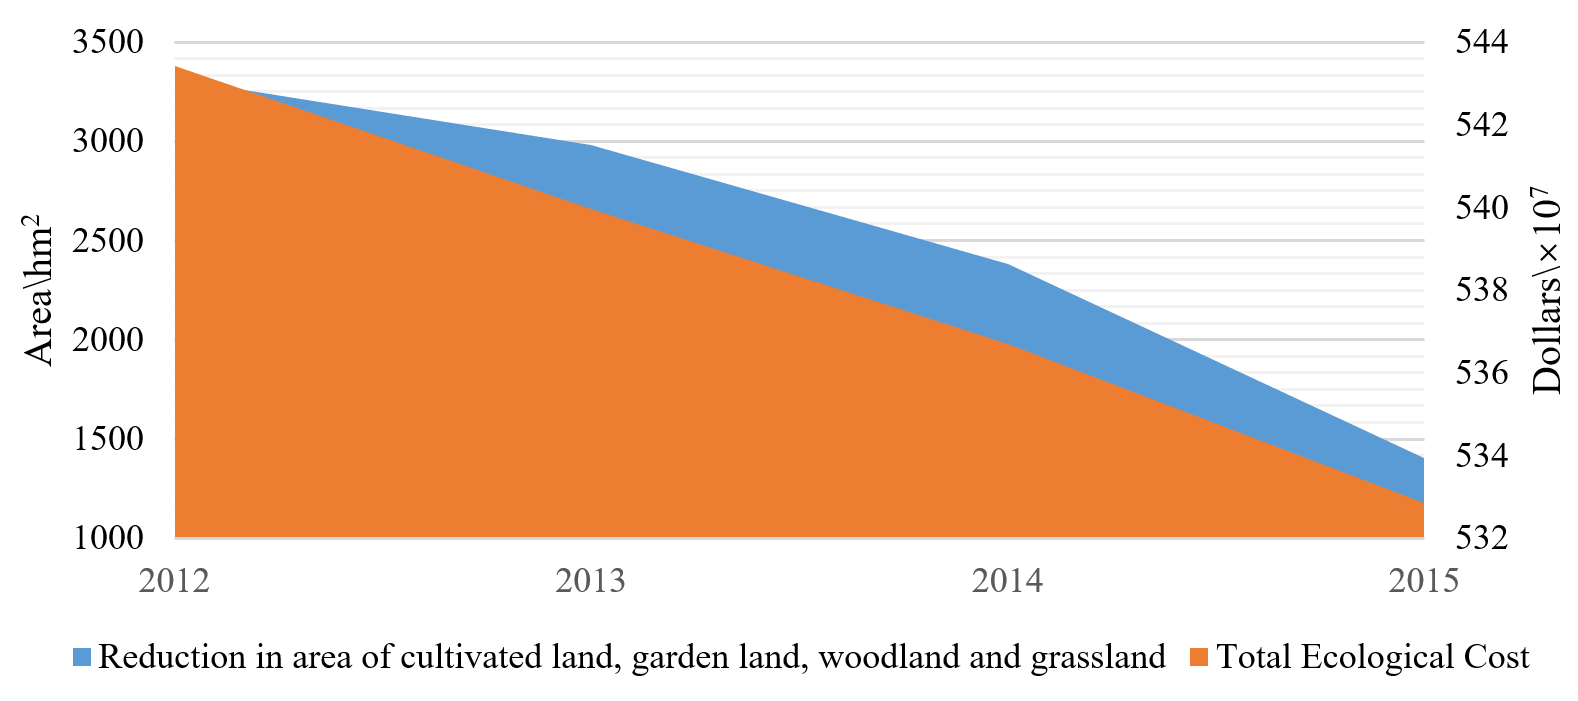
\includegraphics[width=14cm]{nation2.png}
			\caption{Reduction and Total Economic Cost}
			\label{fig:nation2}
		\end{figure}
		
		As shown in the above chart, Beijing's annual environmental costs are decreasing. In the following chart, we analyzed specific indicators to explain the main reasons for Beijing's environmental cost reduction.

		
		\begin{figure}[h]
			\small
			\centering
			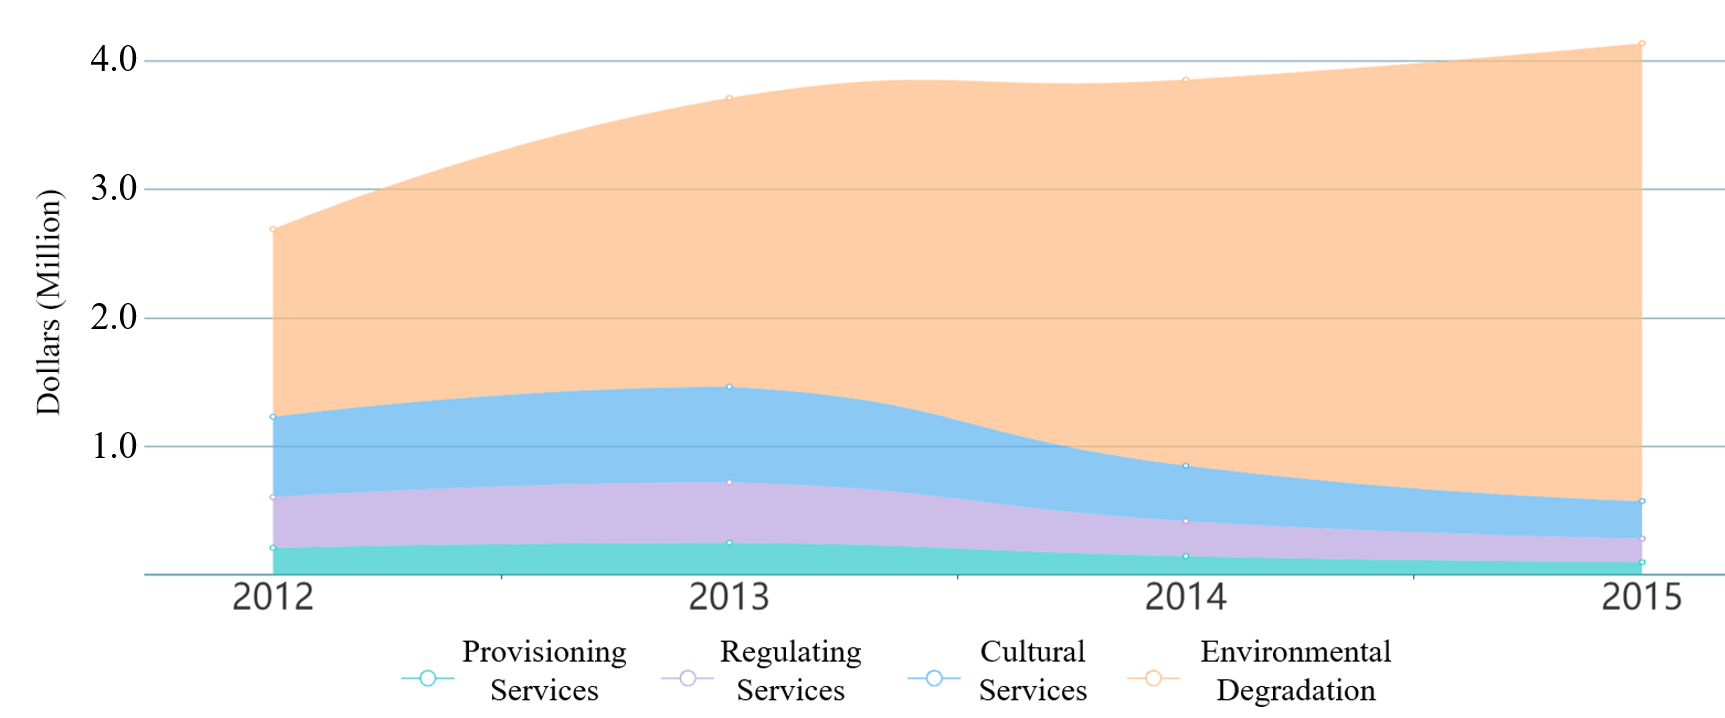
\includegraphics[width=13cm]{nation3.png}
			\caption{Reduction and Total Economic Cost}
			\label{fig:nation3}
		\end{figure}
	
		Using our model, we can calculate the benefit-cost ratio of Beijing as follows:
			
		\begin{table}[h]
			\centering
			\setlength{\tabcolsep}{3.7mm}
			\begin{tabular}{ccc}
				\toprule[1.5pt]  %添加表格头部粗线
				& Without Ecological Cost & With Ecological Cost  \\
				\midrule  %添加表格中横线
				2011& 3.087072902& 1.95413\\
				2012& 5.126588348& 2.729174\\
				2013& 2.947301702& 1.776562526\\
				2014& 3.374446786& 2.063438038\\
				2015& 2.886285606& 1.720510162\\	
				\bottomrule[1.5pt] %添加表格底部粗线
			\end{tabular}
		\end{table}
		
		By analyzing the results of our model output, we find out that with the reduction of annual land declining, the annual increase in the ecological costs of development in Beijing is indeed decreasing, which is in line with our expectation, indicating that our model is effective.
		
		\begin{figure}[h]
			\small
			\centering
			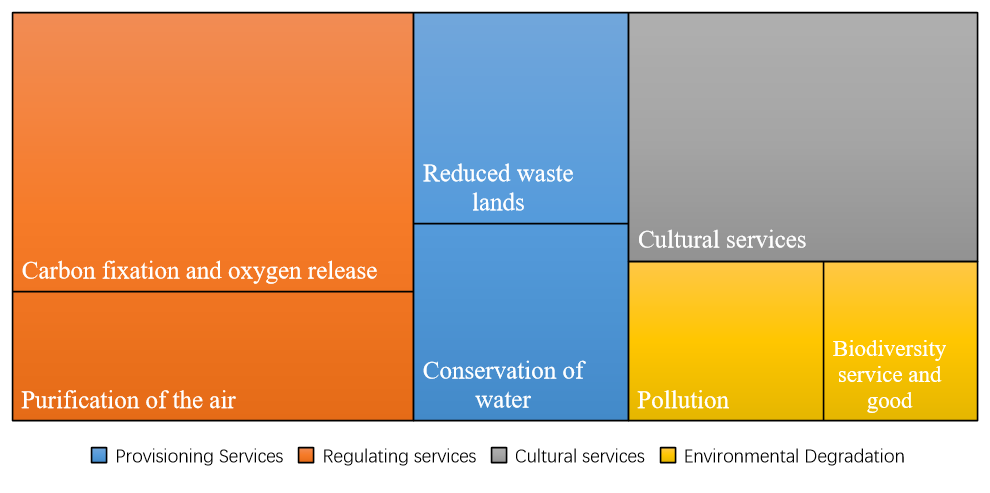
\includegraphics[width=13cm]{nation.png}
			\caption{Large National Project:  Beijing}
			\label{fig:nation}
		\end{figure}
		
		Comparing large projects with small projects, we find out that for small projects, the ecological costs are mainly from pollution, while for large projects (urban development), the proportion of pollution in ecological costs is not high. At the same time, for small projects, the ratio of ecological costs to total costs is far less than that of large projects. After considering environmental costs, the BCR of large projects changes drastically, and ecological costs account for a high proportion of the total cost of large projects. For the development of citys', ecological costs is critical.
		

	\section{Implication on Planners and Managers}		
	
		\subsection{Assumptions}
		
			In order to better understand the application of the model in real life and its implication on land use project managers and planning, we made the following assumptions for further in-depth discussion.
			
			\begin{itemize}
				
				\item \textbf{The planner and manager are the rational economic man.} \\
				Economic man refers to an idealized human being who acts rationally and self-interested, who seeks to maximize personal utility or satisfaction.
				
				\item \textbf{The planner of a land-use project consider economic net present value.} \\
				The planner of a land use project whose primary purpose is to maximize economic benefits, that is to say, will not consider environmental costs, and the secondary purpose is to choose a plan with less environmental costs.
				
				\item \textbf{Managers take environmental cost into account.} \\
				Managers of the city are responsible for choosing planners' projects to implement in cities, so, in the long run, they consider environmental costs as same as accounting cost when selecting projects.
				
				\item \textbf{The market for land use project is a completely competitive market.} \\
				This means that the market will choose projects with high NPV or high BCR.
				
			\end{itemize}
		
		\subsection{Help Planners for Site Selection}
		
			For a project, there are many possible locations, and the different site does not just mean different economic costs, but the various ecological and environmental costs.
			
			A good choice should take care of economic cost and the cost of environmental degradation. Our model can comprehensively evaluate each option, helping planners choose the most appropriate one by comparing the financial costs, ecological costs and overall costs.
		
		\subsection{Help Managers for Urban Planning}
		
			Managers, by using our model and combining with the production possibility boundary,  can know how to plan the use of land resources in order to achieve the best balance between the output of environmental services and the output of economic activities.
			
			In economics, a production–possibility frontier is a curve which shows various combinations of the set of two goods which can be produced with the given resources and technology where the given resources are fully and efficiently utilized.
			
			\begin{figure}[htbp]
				\centering
				\subfigure[]{
					\begin{minipage}[t]{0.5\linewidth}
						\centering
						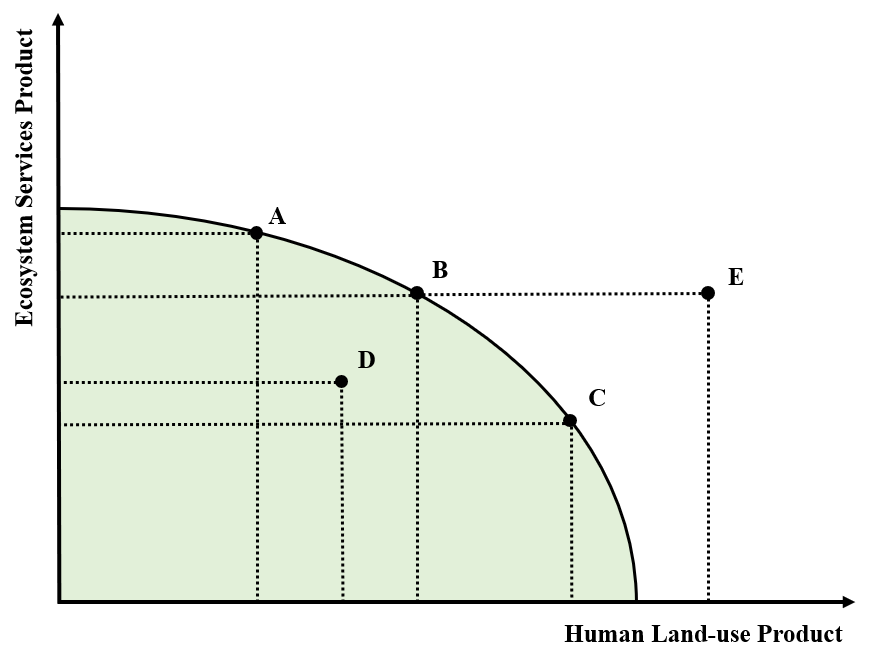
\includegraphics[width=2.5in]{frontier.png}
						%\caption{fig1}
					\end{minipage}%
				}%
				\subfigure[]{
					\begin{minipage}[t]{0.5\linewidth}
						\centering
						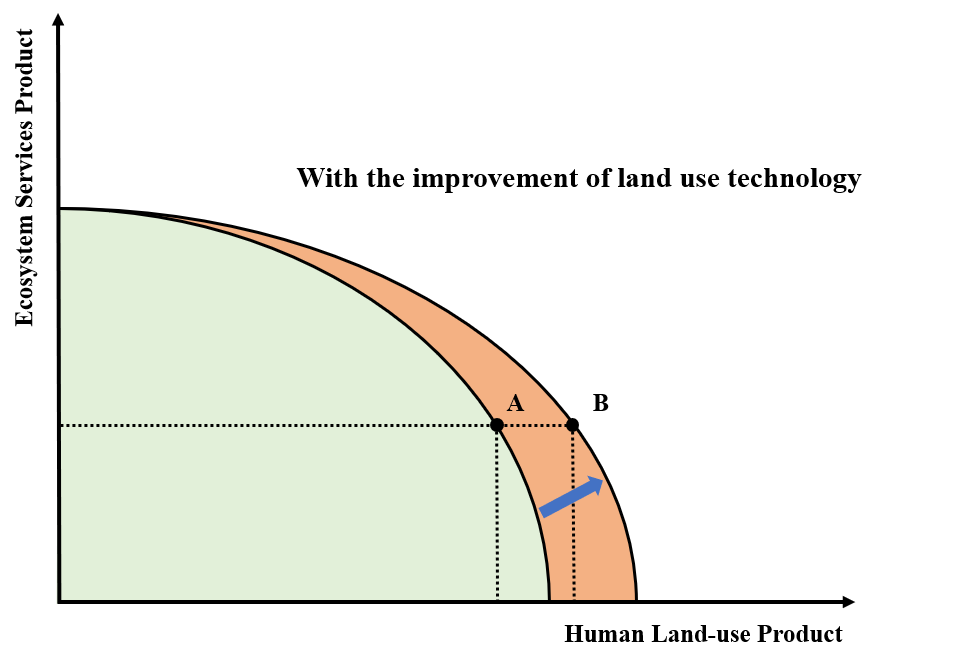
\includegraphics[width=2.5in]{frontier2.png}
						%\caption{fig2}
					\end{minipage}%
				}%
				\centering
				\caption{Production–possibility Frontier between Ecosystem services Product and Human Land-use Product}
			\end{figure}
			
			Take ecological services resources as a product when land is used by ecosystem and take the human project as another product, and let the benefit of the project represents its value. Both of these two products need land resource which is scarce for both human and the world. So a good manager must consider how to achieve the most valuable combination for a city.
			
			A production–possibility frontier can be found for the two products(ecosystem-use and human-use). Each point means a possible combination. The point A and B are on the curve and D is inside the curve. The points on the curve mean that there is no idle land resource and every land is adequately used either by human or ecosystem. These points are the most efficient combinations of resource allocation. These combinations should be managers’ choices. Well the points inside the curve mean that there are land resource left unused. These combinations are the choices that managers that should avoid. And point E is outside the curve because that combination is beyond land resources and present technologies. 
			
			\begin{figure}[h]
				\small
				\centering
				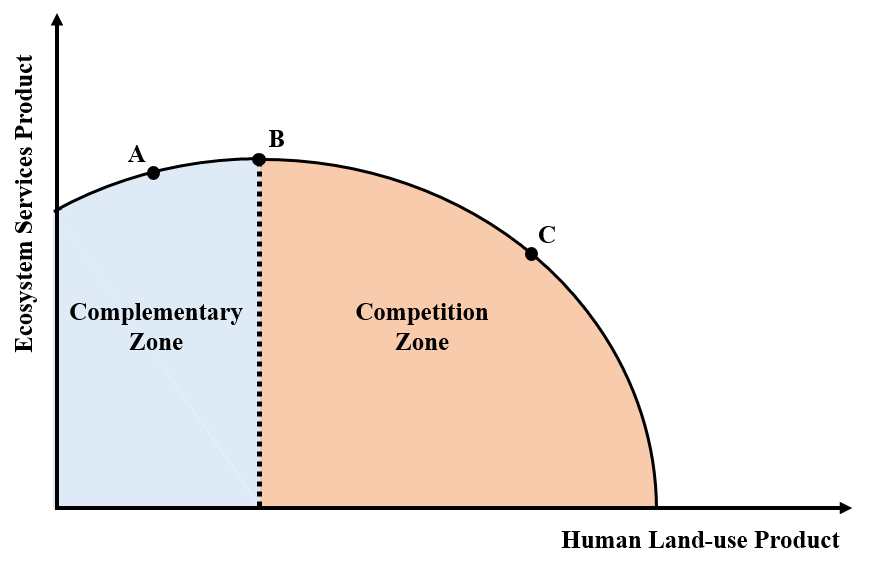
\includegraphics[width=9cm]{frontier3.png}
				\caption{Relationships between Ecosystem Services and Biodiversity}
				\label{fig:multiplier}
			\end{figure}
			
			Interestingly, according to our previous models and analysis, our production possibility boundary is not entirely concave to the origin. The reasons are as follows:
			
			\begin{itemize}
				
				\item \textbf{Moderate human activity may increase ecosystem services by properly reducing  ecological diversity.} According to the conclusion of the literature \cite{de2010challenges}, when the ecological diversity is reduced due to the appropriate interference of human activities, the total ecological services will increase, while excessive human activities will lead to the reduction of the overall ecosystem services.
				
				\item \textbf{The properly combination of human and nature will increase cultural and provisioning services in ecosystem services.} A crucial feature in the valuation of the recreational services of ecosystems is accessibility. The service value, therefore, increases from a low value at primitive systems to high values in friendly light use and subsequent drops to low values for degraded systems. \cite{braat2008cost}.
				
				So the production possibility boundary can be divided into two stages: complementary stage and competitive stage. Such characteristics can help city managers better decide how to balance the conservation of ecosystem services and the development of land use projects.
				
			\end{itemize}
		
	\section{How Model Need to Change over Time?}	
	
		The main reason for the decline in ecosystem services and environmental degradation is the absence of market value. Projects that do not consider environmental costs can lead to negative externalities. In order to incorporate nature into financial accounts, our model provides a viable method and means to monetize natural costs, and over time, the reduction in market externalities will affect the structure of our model, so the market and model are mutual functioning.
		
		\begin{figure}[h]
			\small
			\centering
			
\includegraphics[width=15cm]{externality.png}
			\caption{The relationships among the model, externality and government.}
			\label{fig:externality}
		\end{figure}
		
		Below we will explain in detail how might our model will change over time as the market changes. When the economic value of the environment and ecosystem is quantified, the externalities of the market will be reduced, which means that part of the environmental cost has been included in the economic cost, through the market. We consider two changes in the market that will lead to model changes.
		
		\begin{figure}[htbp]
			\centering
			\subfigure[Present]{
				\begin{minipage}[t]{0.5\linewidth}
					\centering
					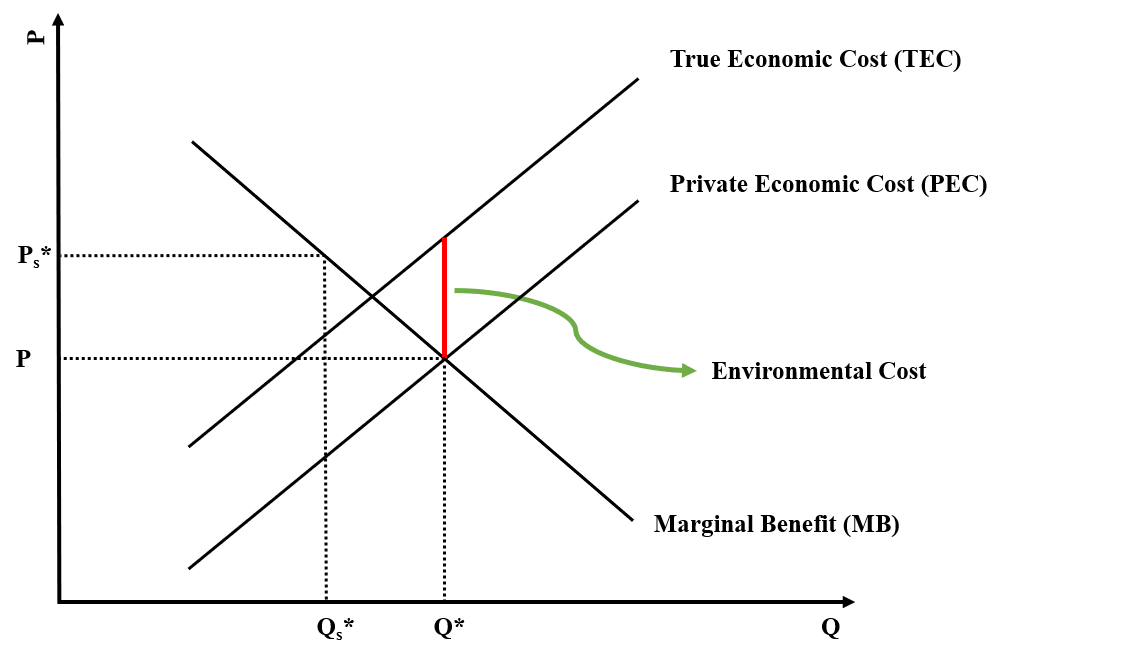
\includegraphics[width=2.5in]{tax.png}
					%\caption{fig1}
				\end{minipage}%
			}%
			\subfigure[Possible Changes over Time]{
				\begin{minipage}[t]{0.5\linewidth}
					\centering
					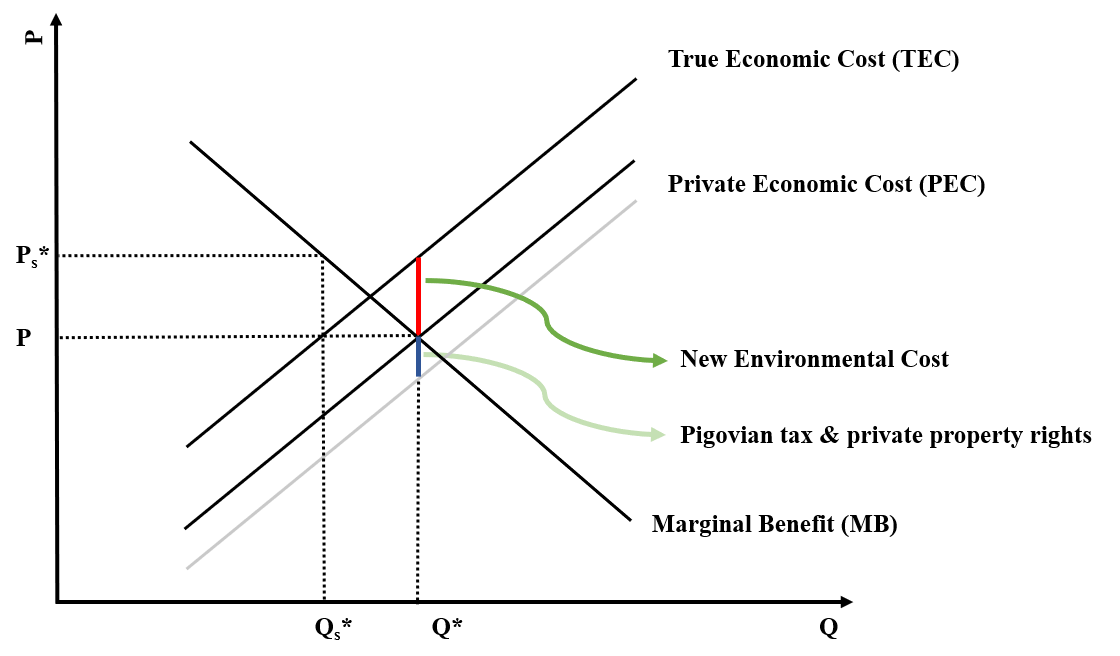
\includegraphics[width=2.5in]{tax2.png}
					%\caption{fig2}
				\end{minipage}%
			}%
			\centering
			\caption{Before and After Considering Changes in the Market}
		\end{figure}
		
		\begin{itemize}
			
			\item \textbf{Pigovian tax \footnote{A Pigouvian tax is a tax on any market activity that generates negative externalities (costs not included in the market price)} placed on the planner}
			
			If planners need to pay taxes for their own environmental degradation, then our model needs to make two changes. \textbf{Let's take fossil fuel tax as an example \footnote{From October 1, 2012, Japan began to impose environmental taxes on fossil fuels such as oil and natural gas.}.} If the government imposed an environmental tax on fossil fuels, the cost caused by fossil fuels has already been reflected in economic costs. To avoid double counting, environmental costs calculated will no longer contain the cost caused by fossil fuels. Instead, the tax is considered when calculating accounting costs.
			
			\item \textbf{Politics of Tradeable Pollution Rights}
			
			Well defined private property rights will makes the  ecosystem no longer a public and non-competitive item. \textbf{We assume that the government forms an emission trading market for $NO_x$ and $SO_x$,} and the pollution is calculated into accounting costs, so they should not be calculated in environmental costs.
			
		\end{itemize}
	
	\section{Sensitivity Analysis}	
	
		In our model, the change of biodiversity multiplier R directly affect ecological costs, so we change R from 1.2 to 0.4 to find out the impact of R in our model.
		
		\begin{figure}[htbp]
			\centering
			\subfigure[Changes in environmental costs]{
				\begin{minipage}[t]{0.5\linewidth}
					\centering
					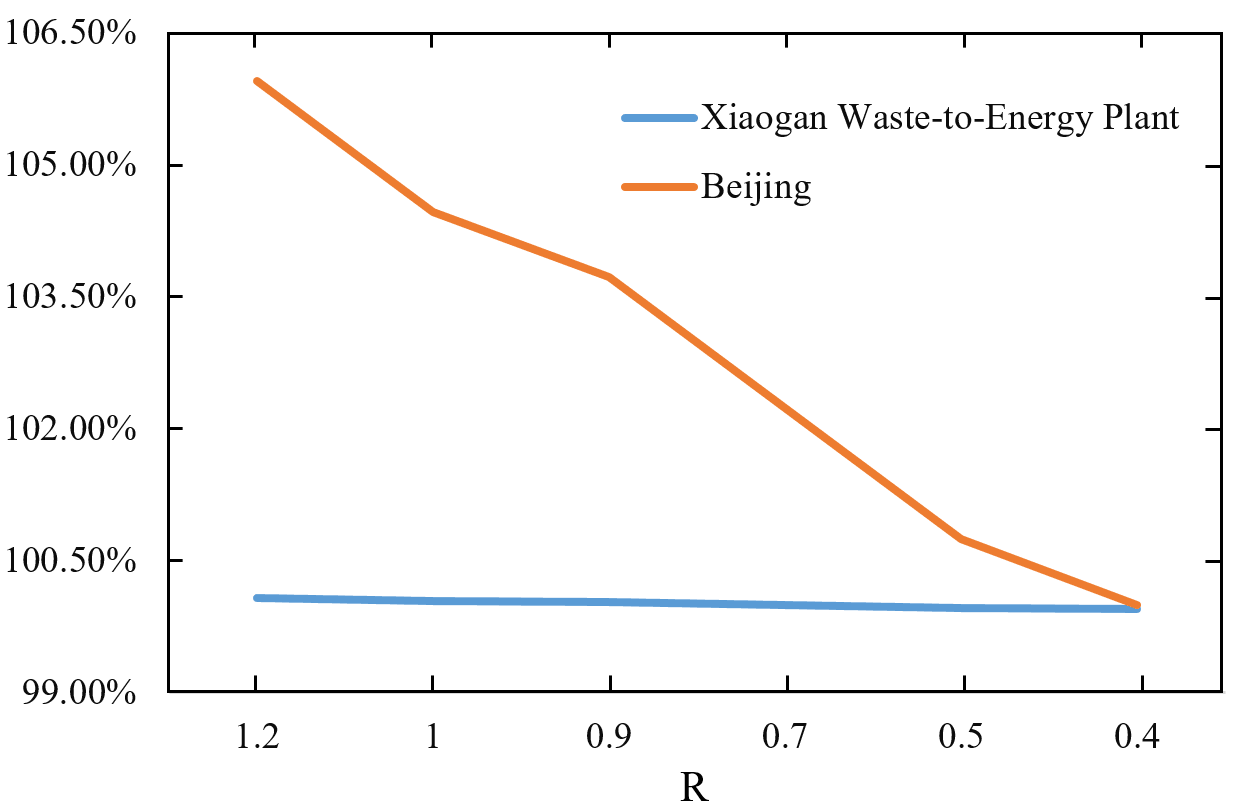
\includegraphics[width=2.5in]{left.png}
				\end{minipage}%
			}%
			\subfigure[Changes in BCR]{
				\begin{minipage}[t]{0.5\linewidth}
					\centering
					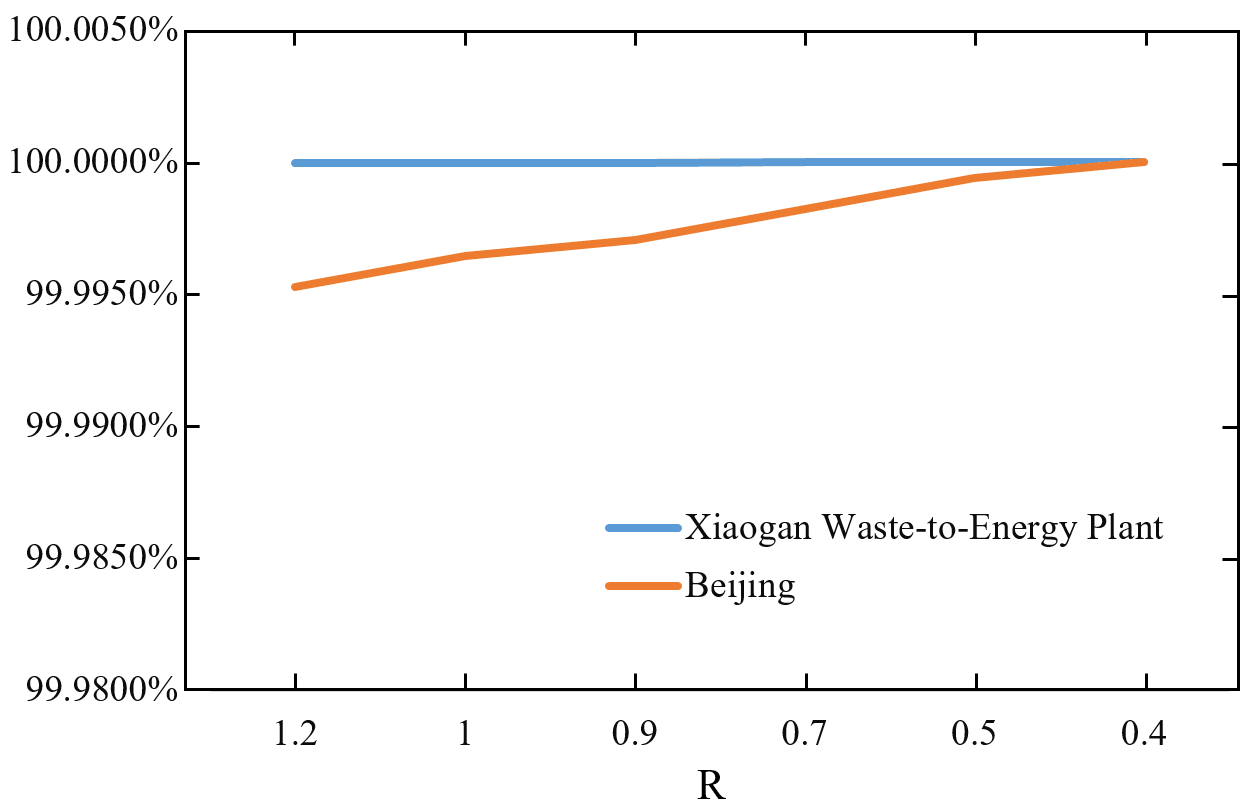
\includegraphics[width=2.5in]{right.png}
				\end{minipage}%
			}%
			\centering
			\caption{The impact of changes in R on environmental costs and BCR}
		\end{figure}
		
		The left figure shows the change rate of ecological costs of two projects under different R. The result shows that the change of R has a greater impact on the ecological costs of Beijing, but a smaller impact on Xiaogan waste-to-energy plant. This is because for small projects, Xiaogan waste-to-energy plant has a small proportion of ecosystem services, while R directly affects the cost of ecosystem services, so R has a small impact on the ecological costs of Xiaogan waste-to-energy plant. For large projects, Beijing has a large proportion of ecosystem services, so R has a great impact on the ecological costs of Beijing.
		
		The right figure shows the change rate of BCR of two projects under different R. For the two projects, the proportion of internal costs is much higher than the ecological costs, while R can only affect part of the ecological costs, so the impact of R on BCR is very small. On the basis of this, R has a greater impact on BCR of Beijing than Xiaogan waste-to-energy plant.
		
	
	\section{Strengths and Weaknesses}
	
		\subsection{Strengths}
		
			\begin{itemize}
				
				\item \textbf{Wide application}\\Our model takes a lot of factors into consideration so that it can be applied to plenty of situations.
				
				\item \textbf{Objective and Persuasive}\\We measure various kinds of ecosystem services value in different mathematics or economics methods. And these objective methods are widely used in other models.
				
				\item \textbf{Vivid}\\We use various kinds of charts to explain our process and show our views and conclusions.

	
			\end{itemize}
		
		\subsection{Weaknesses}
		
			\begin{itemize}
				
				\item \textbf{Lack of data}\\
				We neglect some indicators such as energy because we lack an accurate database, which may result in notable errors of some specific land-use projects.
				
				\item \textbf{Double counting}\\
				There are interactions between environmental indicators. So when we calculate the ecological costs, our model may cause double counting.
		
			\end{itemize}
		
	\section{Conclusions and Future Work}
	
	
		\subsection{Conclusions}
	
			We build an environmental cost valuation model to analyse the true economic costs of land-use projects, considering the aspects of ecosystem services and environmental degradation. 
			
			We employ different mathematical and economic methods to measure various indicators' economic costs. Then we use our model to perform a cost-benefit analysis on Beijing and a waste-to-power plant. we come to the conclusion that among the environmental costs of small scale projects, pollution is the culprit. And large projects should be alert to excessive damage to the ecosystem services.
			
			Implications of our modelling on land use project planners and managers is discussed next. The planner can choose the focus to consider as needed for their site selection. The managers should find the suitable project's combination based on the production-possibility frontier. 
			
			Then we discussed why our model might need to change in the future: the externalities of the market continue to decrease with the implementation of national policies. Finally, we do sensitivity analysis, discuss strengths and weaknesses and prove the credibility of our model.
			
		\subsection{Future Work}
		
			There are several drawbacks in our model, such as the double counting problem. We need to do more to improve our work.
			
			\begin{itemize}
				
				\item \textbf{Handling of different country scenarios}\\
				Different countries have different economic management measures, and different policies are adopted for environmental pollution. These will affect the accuracy of the model. There is no unified model that can perfectly calculate the environmental costs of all countries, so special circumstances need special treatment.
				
				\item \textbf{Market characteristics}\\
				We assume that the land use market is completely competitive. The actual situation is not always the case. When the land use market is an oligopolistic market or a monopolistic competitive market, the cost calculation will be different and we need to consider it separately.
				
			\end{itemize}
	
	\newpage
		
	\nocite{*}
	\bibliographystyle{unsrt}
	\bibliography{reference.bib}	
	\newpage


\end{document}



